%!TEX root = thesis.tex
\chapter{Results}
\section{Charm baryon production}
\subsection{\Lc and \Sc measurements}
ALICE has measured all single-charm hadron ground states in pp collisions, including charm mesons ($\rm D^{0}$, $\rm D^{+}$, $\rm D_{s}^{+}$) at \tevf~\cite{nonpromptD} and charm baryons (\Lc, $\rm \Xi_{\rm c}^{0,+}$ and \Oc) at \tevf and \tevt~\cite{Acharya:2020uqi,alicecollaboration2021measurement}.
In addition, ALICE measured \Lc in p--Pb collisions at $\sqrt{s_{\rm NN}} = 5.02\,\rm TeV$  down to \pt = 0. 

The \Lc/\Do ratios in pp and p--Pb collisions at $\sqrt{s_{\rm NN}} = 5.02\,\rm TeV$ are shown in the Fig.\ref{LcFig}.
At low \pt, the \Lc/\Do ratio measured in p--Pb collisions was significantly lower than in pp collisions, and at intermediate \pt, the \Lc/\Do ratio measured in p--Pb collisions was higher with respect to the one measured in pp collisions.
This modification can be interpreted as due to the radial flow or additional hadronisation process in p--Pb collisions.
\begin{figure}[ht!]
    \centering
    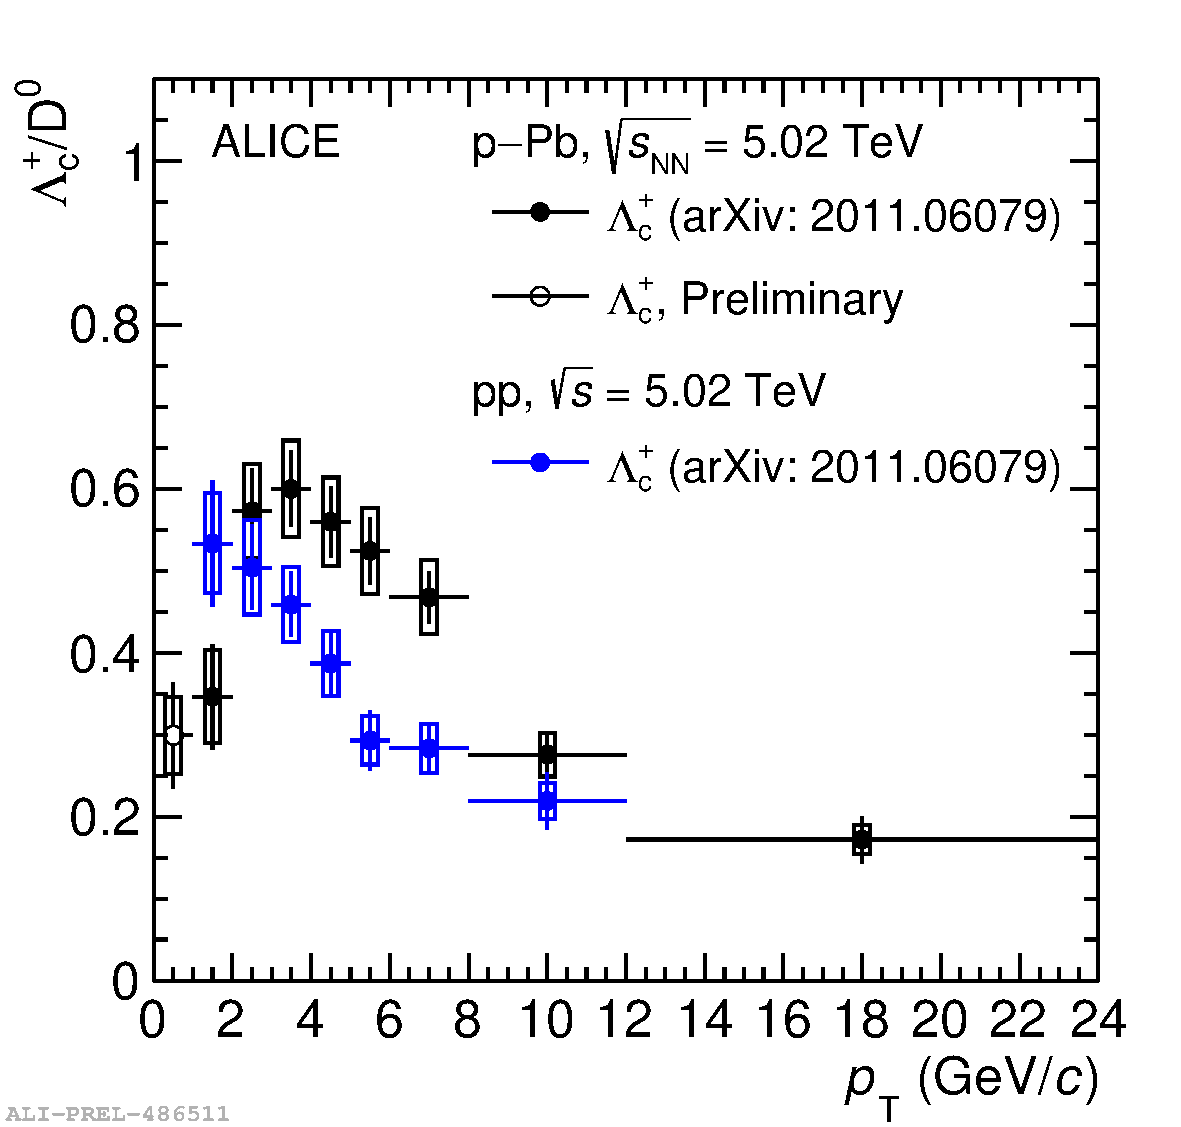
\includegraphics[width=0.85\textwidth]{fig/LcD0_Comparison_pp_pPb.pdf}
    \caption{\it $\Lambda_{\rm c}^{+}/D^{0}$ as a function of \pt in pp and p--Pb collisions at \tevf.}
    \label{LcFig}
\end{figure}

The \Sc/\Do ratio measured in pp collisions at \tevt is shown in the Fig.\ref{ScFig}.
The model calculation from PYTHIA8 Monash ~\cite{Skands:2014pea} largely underestimates the measurement, the statistical hadronisation model (SHM) with excited charm baryon states predicted by the relativistic quark model (RQM) ~\cite{Andronic:2009sv} can describe the measurement within uncertainties.
The model calculations of Catania~\cite{MINISSALE2021136622} and quark (re-)combination mechanism (QCM)~\cite{Song:2018tpv} both including the coalescence process, also can describe the measurement. In general, PYTHIA8 implemented colour reconnection beyond the leading-colour approximation (CR-BLC)~\cite{Christiansen:2015yqa} better describes the \Lc/\Do ratio and \Sc/\Do ratio, which do not contain the strange quarks.
\begin{figure}[ht!]
    \centering
    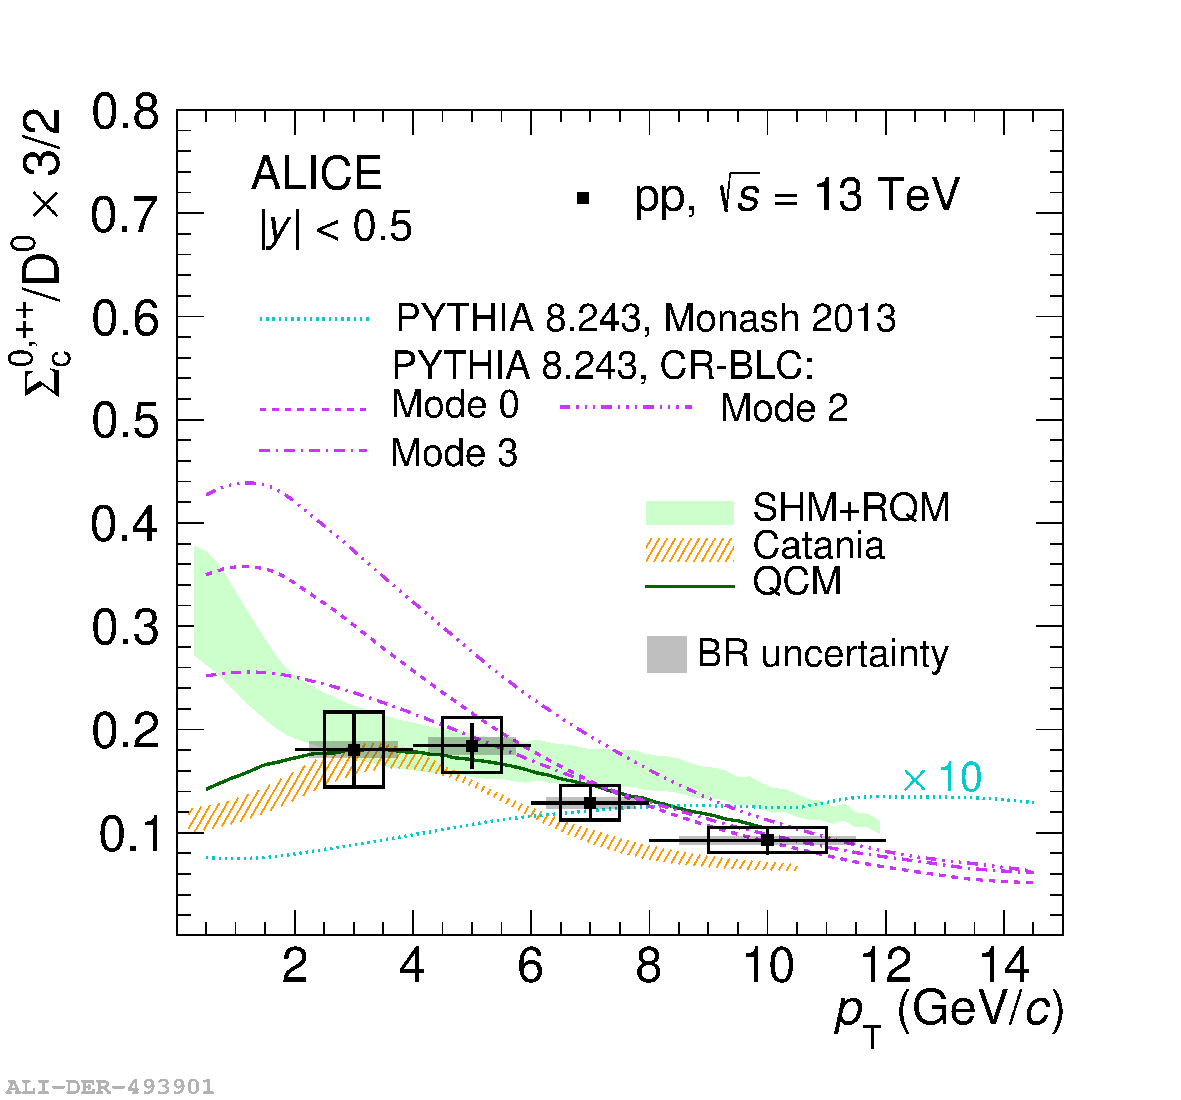
\includegraphics[width=0.85 \textwidth]{fig/plot_scd0.pdf}
    \caption{\it $\rm \Sigma_c^{0,++}/D^{0}$ ratio as a function of \pt at \tevt.}
    \label{ScFig}
\end{figure}



\subsection{\Xiczp and \Oc measurements}
The $\rm \Xi_c^0/D^0$ and $\rm \Xi_c^{+}/D^0$ ratio are shown in the Fig.\ref{XicFig}.
Most of the model calculations significantly underestimate the $\Xi_{\rm c}/{\rm D^0}$ ratio.
However, the Catania model describes better the ratios in the measured \pt interval.
It means that both fragmentation and coalescence processes are important in pp collisions for the hadronisation process.
\begin{figure}[ht!]
    \centering
    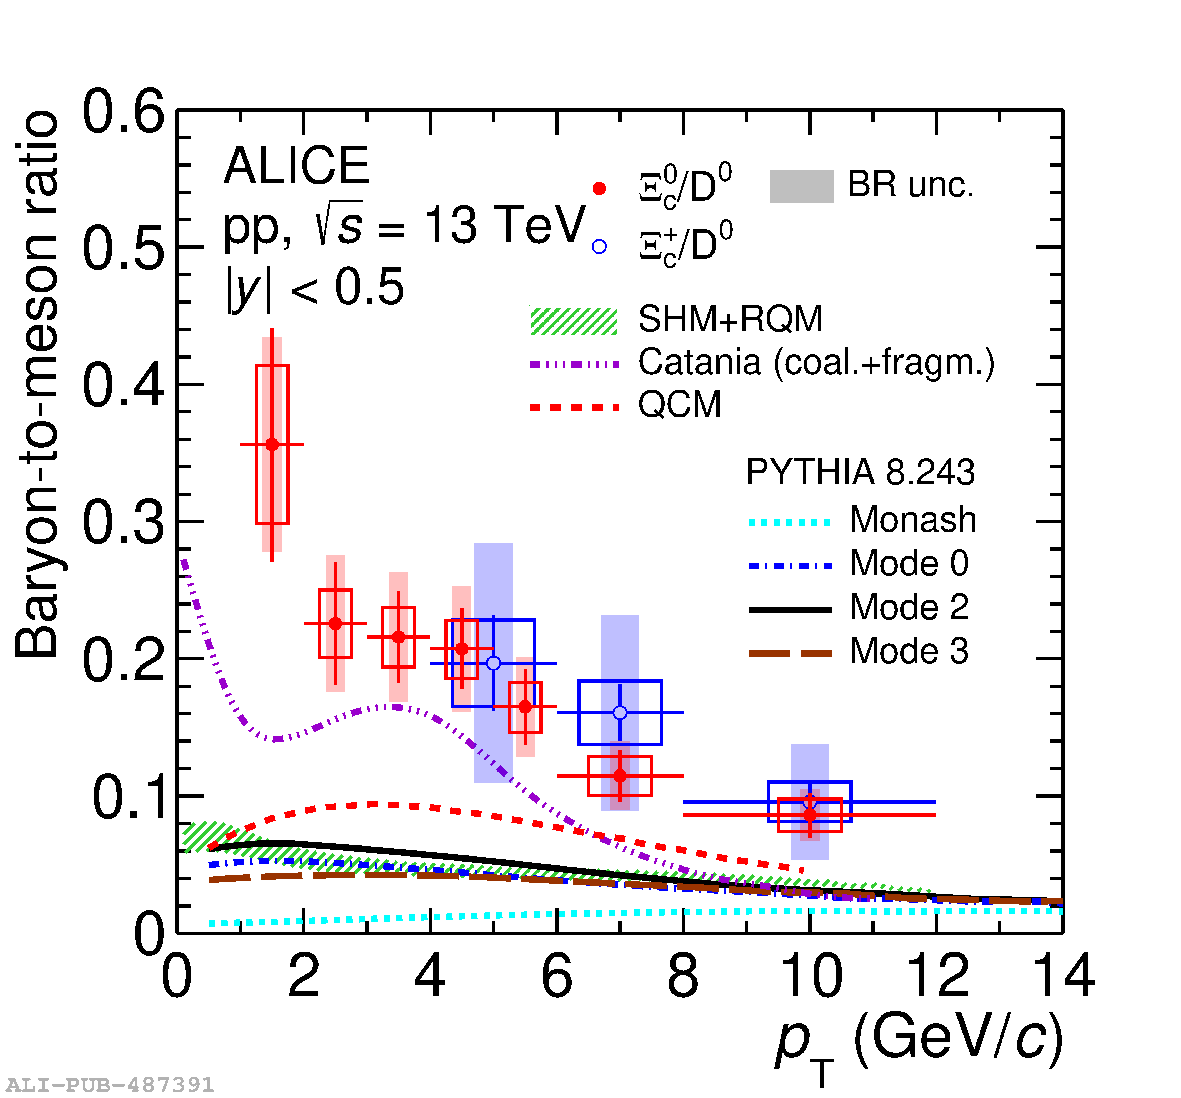
\includegraphics[width=.85\textwidth]{fig/Xic0ToD0_pp13TeV_wModel-3.pdf}
    \caption{\it $\rm \Xi_c^0/D^0$ and $\rm \Xi_c^{+}/D^0$ ratio as a function of \pt at \tevt.}
    \label{XicFig}
\end{figure}

The $\rm BR(\rm \Omega_c^{0} \rightarrow \Omega^{-} \pi^{+})$ $\times$ $\sigma(\Omega_{\rm c}^{0})/\sigma(D^{0})$ ratio is shown in the Fig.\ref{OcFig}.
The branching ratio of $\rm \Omega^{0}_{\rm c} \rightarrow \Omega^{-} \pi^{+}$ is not measured yet, the theoretical calculation of \BR$(\rm \Omega^{0}_{\rm c} \rightarrow \Omega^{-} \pi^{+})$~\cite{Hsiao_2020} is used to scale the model predictions.
Most of the models underestimate the measurements. The Catania model is the calculation that gets closer to the measurements of the $\rm \Xi_c^0/D^0$ and $\rm \Xi_c^{+}/D^0$ ratio and the $\rm BR(\rm \Omega_c^{0} \rightarrow \Omega^{-} \pi^{+})$ $\times$ $\sigma(\Omega_{\rm c}^{0})/\sigma(D^{0})$ ratio.
\begin{figure}[ht!]
    \centering
    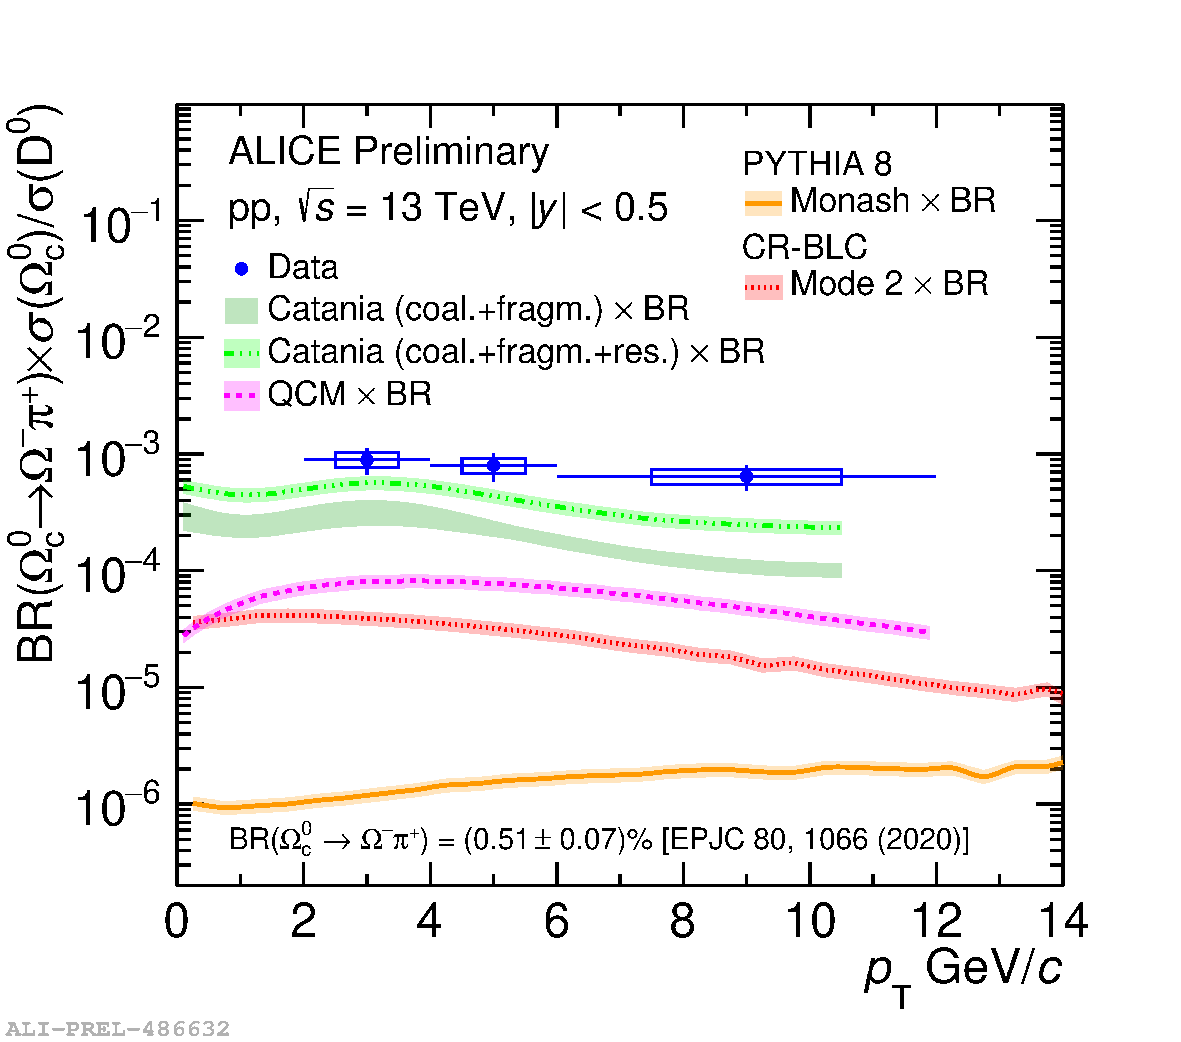
\includegraphics[width=.85\textwidth]{fig/brxomegac0tod0_pp13tev_wmodel_0.pdf}
    \caption{\it BR($\rm \Omega_c^{0} \rightarrow \Omega^{-} \pi^{+}$) $\times \rm \Omega_c^0/D^0$ ratio as a function of \pt at \tevt.}
    \label{OcFig}
\end{figure}


\section{Charm fragmentation fractions}
\subsection{Charm fragmentation fractions}
The charm fragmentation fractions are measured in pp collisions at \tevf.
The numbers are presented in the Table \ref{tab:ccf}
The fragmentation fraction for the \Xicz baryon is measured for the first time.
The contribution of \Xicp is considered by doubling the \Xicz yield since they are isospin partners.
The \Oc is not measured at this energy, so the contribution is included in the systematic uncertainty.
The charm fragmentation fractions measured in pp collisions are compared with \ee and ep measurements in the Fig.\ref{cff}.
The charm fragmentation fractions measured in pp collisions at the LHC are different from the ones measured in \ee and ep collisions, showing that the universality of parton-to-hadron fragmentation is not valid.
\begin{table}
	\begin{center}
		\begin{tabular}{ c c}
		$\rm H_{\rm c}$ & $f(c \rightarrow \rm H_{\rm c})[\%]$ \\
		\hline
        \vspace{0.3cm}
		\ $\rm D^{0}$ & $39.1 \pm 1.7(\rm stat)^{+2.5}_{-3.7}(\rm syst)$ \\
        \vspace{0.3cm}
        \ $\rm D^{+}$ & $17.3 \pm 1.8(\rm stat)^{+1.7}_{-2.1}(\rm syst)$ \\
        \vspace{0.3cm}
        \ $\rm D^{+}_{\rm s}$ & $7.3 \pm 1.0(\rm stat)^{+1.9}_{-1.1}(\rm syst)$ \\
        \vspace{0.3cm}
        \ \Lc & $20.4 \pm 1.3(\rm stat)^{+1.6}_{-2.2}(\rm syst)$ \\
        \vspace{0.3cm}
        \ \Xicz & $8.0 \pm 1.2(\rm stat)^{+2.5}_{-2.4}(\rm syst)$ \\
        \vspace{0.3cm}
        \ $\rm D^{*+}$ & $15.5 \pm 1.2(\rm stat)^{+4.1}_{-2.9}(\rm syst)$ \\
		\end {tabular}
	\caption {\it Charm quark fragmentation fractions into charm hadrons.}
	\label{tab:ccf}
	\end{center}
\end{table}

\begin{figure}[ht!]
    \centering
    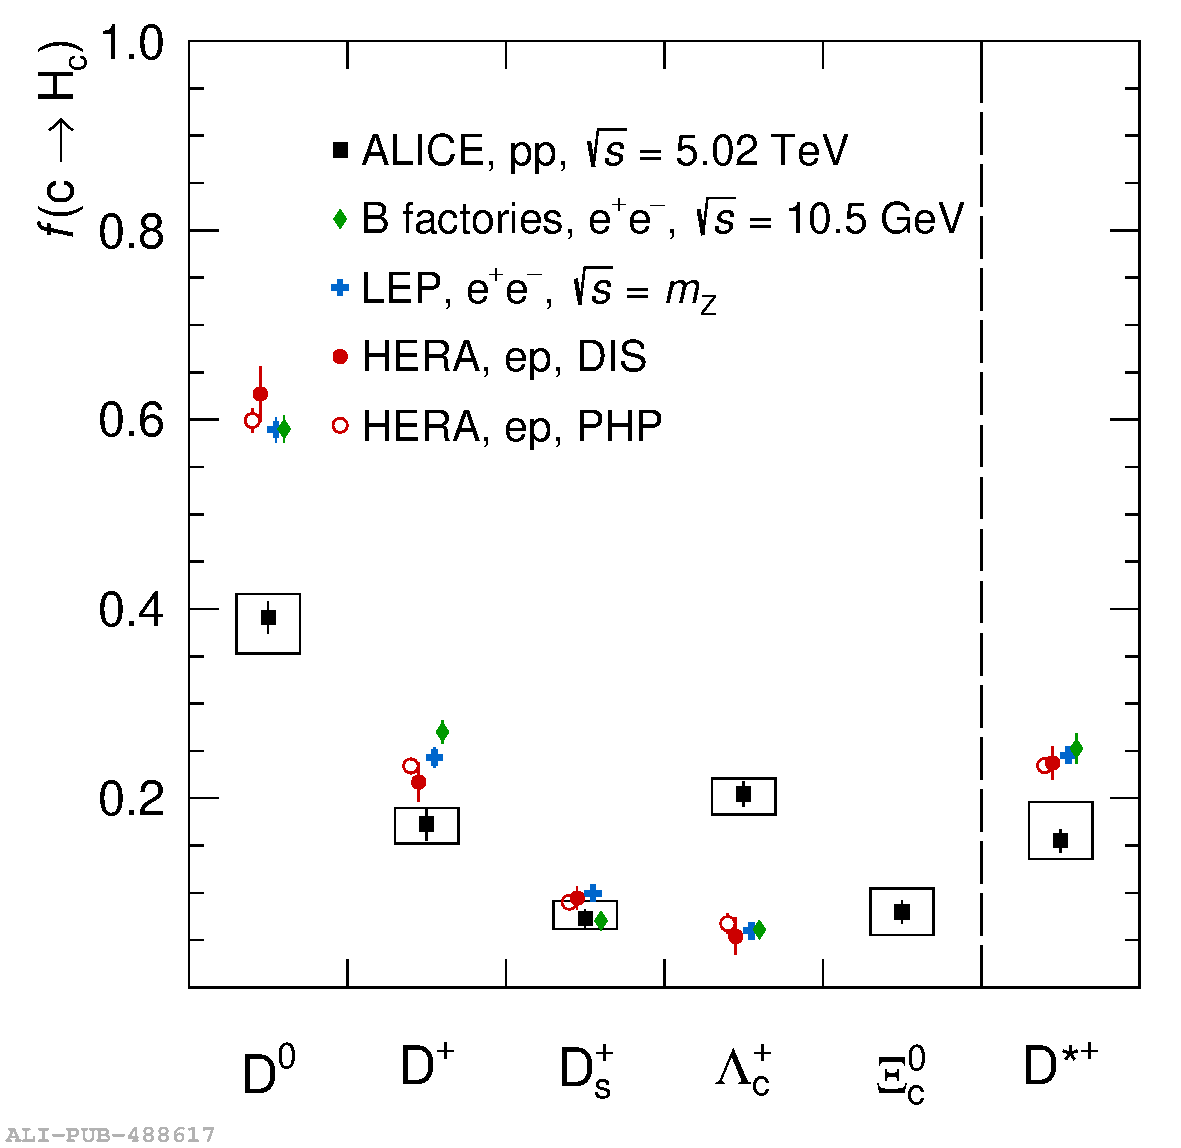
\includegraphics[width=.85\textwidth]{fig/FF5tev.pdf}
    \caption{\it Charm-quark fragmentation fractions into charm hadrons in pp collisions at \tevf compared to the measurements in \ee and ep collisions.}
    \label{cff}
\end{figure}


\subsection{Charm production cross sections}
The charm production cross sections at midrapidity per unit of rapidity are shown in the Fig.\ref{ccbar}.
The charm cross section per unit of rapidity in pp collisions at \tevf is measured at the LHC for the first time, resulting in the \ref{for1}.
\begin{equation}
    {{\rm d\sigma^{\rm c\bar c}}/{\rm dy|^{\rm pp, 5.02 TeV}_{|y|<0.5}} = 1165 \pm 44(\rm stat)^{+134}_{-101}(\rm syst) \mu \rm b}
    \label{for1}
\end{equation}
According to the new measured charm fragmentation fractions, the charm cross section measurements in pp collisions at $\sqrt{s} = 2.76\,\rm TeV$~\cite{Abelev_2012} and $7 \,\rm TeV$~\cite{Acharya_2017} are updated and are about 40\% higher than the previously published results.
The measurements with new charm fragmentation fractions lie at the upper edge of the pQCD calculations~\cite{Cacciari:1998it,PhysRevLett.118.122001}.
\begin{figure}[ht!]
    \centering
    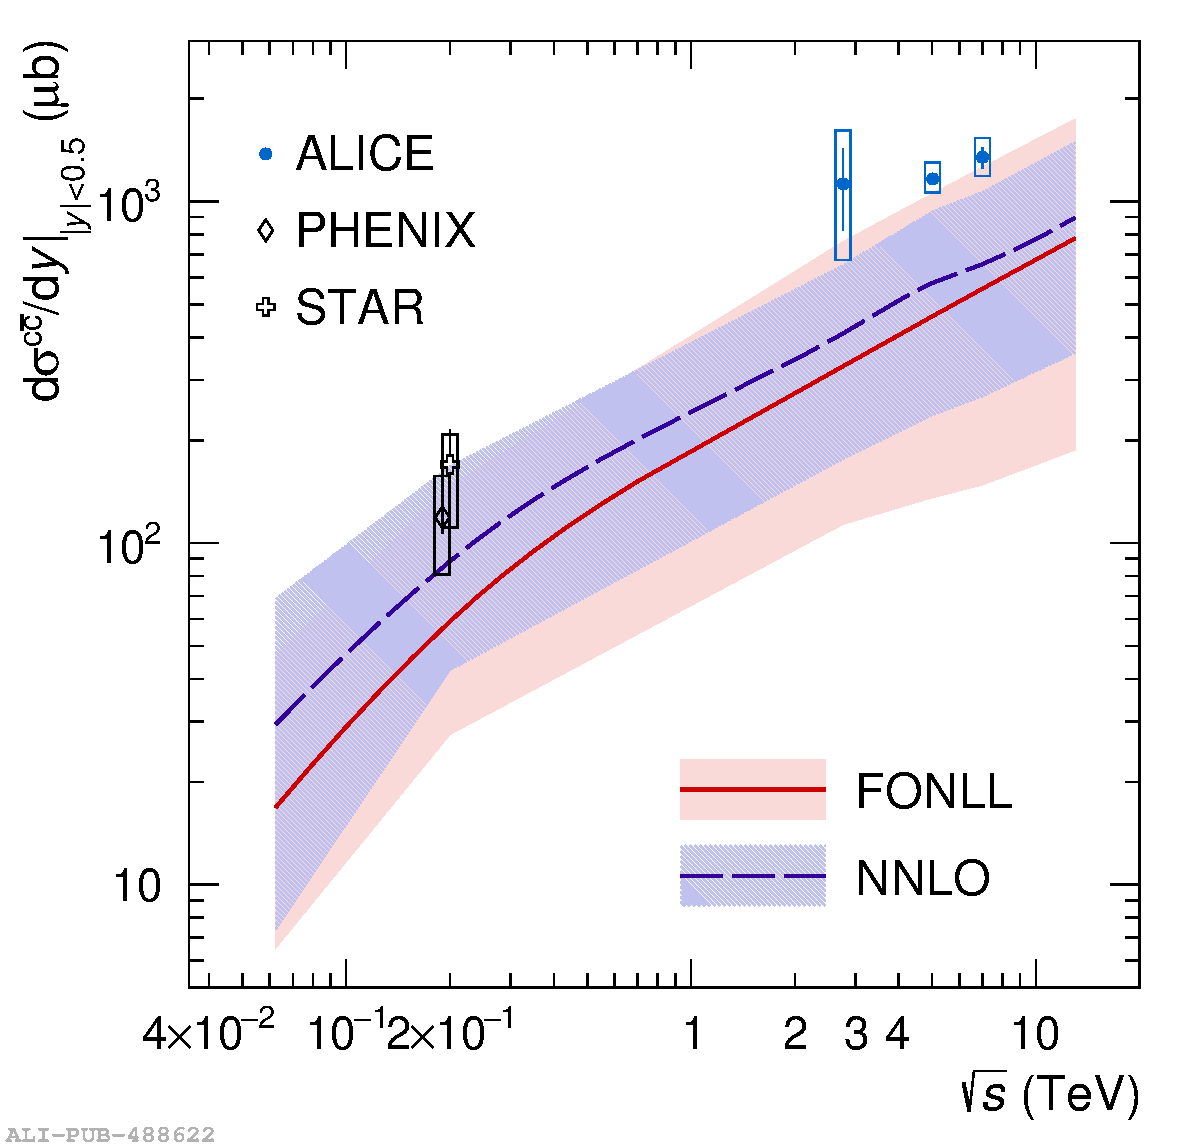
\includegraphics[width=.85\textwidth]{fig/cc_Vs_energy.pdf}
    \caption{\it Charm production cross section at midrapidity as function of the collision energy.}
    \label{ccbar}
\end{figure}